\documentclass[a4paper,12pt]{report}
\usepackage[a4paper, portrait, margin=0.5in]{geometry}
\usepackage[utf8]{inputenc}
\usepackage{graphicx}
\usepackage{dsfont}
\usepackage{amsmath}
\usepackage{esint}
\usepackage{mathtools}
\usepackage{cancel}
\usepackage{bbold}
\usepackage{wrapfig}
\usepackage{subcaption}
\usepackage{listings}
\usepackage{xcolor}		
\usepackage{systeme}
\usepackage{soul}
\usepackage{ amssymb }

\setcounter{secnumdepth}{3}
\setcounter{tocdepth}{3}

\newcommand{\limit}[2]{\underset{#1 \rightarrow #2}{\lim} \,}
\newcommand{\arrowlim}[2]{\overset{#1 \rightarrow #2}{\longrightarrow}}
\newcommand{\arrowlimtwo}[4]{\overset{\scriptsize{\begin{array}{cc}
				#1 {}&\rightarrow #2\\
				#3 &\rightarrow #4
		\end{array}}
	}{\longrightarrow}}

\newcommand{\Lagr}{\mathcal{L}}
\newcommand{\Four}{\mathcal{F}}
\newcommand{\TdZ}{\mathcal{Z}}
\newcommand{\R}{\mathbb{R}}
\newcommand{\C}{\mathbb{C}}
\newcommand{\N}{\mathbb{N}}
\newcommand{\Z}{\mathbb{Z}}
\newcommand{\nextpassage}{\nonumber \\ &\downarrow \nonumber \\}
\newcommand{\firstpassage}{ \\ &\downarrow \nonumber \\}
\newcommand{\spacer}{\quad ; \quad}
\newcommand{\except}[1]{\backslash \{ #1 \} }
\newcommand{\taleche}{\; : \;}
\newcommand{\bolditem}[1]{\item \textbf{#1}}
\newcommand{\separator}{\nonumber \\ 
	\nonumber \\}
\newcommand{\double}[2]{\left\{ \begin{array}{cc}
		#1\\
		#2
	\end{array}
	\right.
}
\newcommand{\triple}[3]{\left\{ \begin{array}{ccc}
		#1\\
		#2\\
		#3
	\end{array}
	\right.
}	
\newcommand{\quadruple}[4]{\left\{ \begin{array}{ccc}
		#1\\
		#2\\
		#3\\
		#4
	\end{array}
	\right.
}	

\newcommand{\nosgn}{\;\;\,}

\newcommand{\quadvec}[4]{\left( \begin{array}{ccc}
		#1\\
		#2\\
		#3\\
		#4
	\end{array}
	\right)
}

% Title Page
\title{Studio di un circuito a doppia maglia LC}
\author{Alessandro Marcelli}


\begin{document}
\maketitle
\tableofcontents
\begin{abstract}
\end{abstract}

\section{Il circuito LCLC ideale}
Un circuito a doppia maglia LC ideale si presenta nel seguente modo
\begin{figure}[!htb]
	\centering
	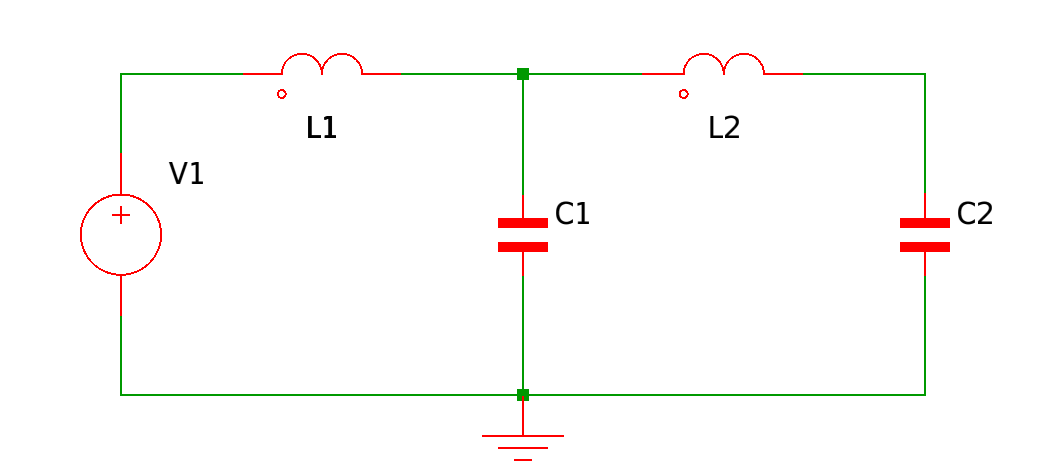
\includegraphics[width=\textwidth]{pictures/schemaideale.png}
	\label{fig:largenenough}
	\caption{\label{lul} \small LCLC ideale}
\end{figure}

Con $L_1 = L_2$ e $C_1 = C_2$. Lo si può risolvere in diversi modi (Metodo dei nodi, delle maglie, Thevenin), ma in definitiva si otterà che
\begin{align}
v_{out} = \frac{1}{(1 - \omega^2 LC )^2 - \omega^2LC}\cdot v_{in}
\end{align}

E quindi si avrà la funzione di trasferimento del circuito come

\begin{align}
H(\omega) = \frac{v_{out}}{v_{in}} = \frac{1}{(1 - \omega^2 LC )^2 - \omega^2LC}
\end{align}

Osservando la forma della funzione di trasferimento possiamo notare come siamo in presenza di un circuito che filtra il segnale in ingresso, eliminando i segnali a frequenze più alte, ovvero abbiamo un filtro \textbf{Passa-Basso}.

Definendo la \textbf{pulsazione di risonanza del circuito} come
\begin{align}
\omega_0 = \frac{1}{\sqrt{LC}}
\end{align}

Possiamo esprimerne i poli come
\begin{align}
\omega_1 = 0.618 \cdot \omega_0 \spacer \omega_2 = 1.618 \cdot \omega_0
\end{align}

\newpage

\subsection{Analogie con la linea di trasmissione e adattamento in potenza del filtro}

Lo studio di circuiti a maglie LC presenta analogie con la trattazione a parametri concentrati della linea di trasmissione. Ci si può quindi aspettare che ponendo in parallelo a $C_2$ un carico resistivo del valore
\begin{align}
R_L = \sqrt{\frac{L}{C}}
\end{align}

le oscillazioni in prossimità dei poli della funzione di trasferimento vengano fortemente smorzate, assorbendo il carico gran parte del segnale e riducendo le riflessioni di segnale interne al filtro che comportano le esplosioni in ampiezza in corrispondenza dei poli.

\section{Simulazione su SIMetrix del circuito ideale}

Scopo della simulazione è quello di studiare il comportamento del circuito in due situazioni:
\begin{enumerate}
\item Circuito non adattato
\item Circuito con resistenza di adattamento ai capi dell'uscita
\end{enumerate}

\subsection{Calcolo a priori della frequenza di risonanza e dei poli della funzione di trasferimento}

Si è simulato su SIMetrix un circuito a doppia maglia LC utilizzando componenti con i seguenti valori
\begin{align}
&L_1 = L_2  = L= 4.7 \; [mH]\\ 
&C _1 = C_2 = C = 200 \; [pF]
\end{align}

Ci si aspetta quindi una frequenza di risonanza pari a
\begin{align}
\omega_0 = \frac{1}{\sqrt{LC}} = \frac{1}{\sqrt{4.7 \cdot 10^{-3} \cdot 200 \cdot 10^{-12}}} \simeq 1.031 \cdot 10^6 \; \frac{[rad]}{[s]}
\end{align}


Ci si aspettano quindi dei poli in
\begin{align}
&\omega_1 = 0.618 \cdot \simeq 1.031 \cdot 10^6 \; \frac{[rad]}{[s]} = \simeq 6.37 \cdot 10^5 \; \frac{[rad]}{[s]}\\
&\omega_2 = 1.618 \cdot \simeq 1.031 \cdot 10^6 \; \frac{[rad]}{[s]} = \simeq 16.7 \cdot 10^5 \; \frac{[rad]}{[s]}
\end{align}

Convertiamo in Hertz per comodità, essendo l'unità di misura utilizzata da SIMetrix
\begin{align}
&\omega_1 = 101,382 \; [kHz]\\
&\omega_2 = 265,788 \; [kHz]
\end{align}

\newpage

\subsection{Simulazione del circuito ideale non adattato in potenza}

Si è simulato il circuito ideale inserendo le componenti prima indicate, e si è posta una probe per i plot di Bode agli estremi del circuito, come si vede di seguito.
\begin{figure}[!htb]
	\centering
	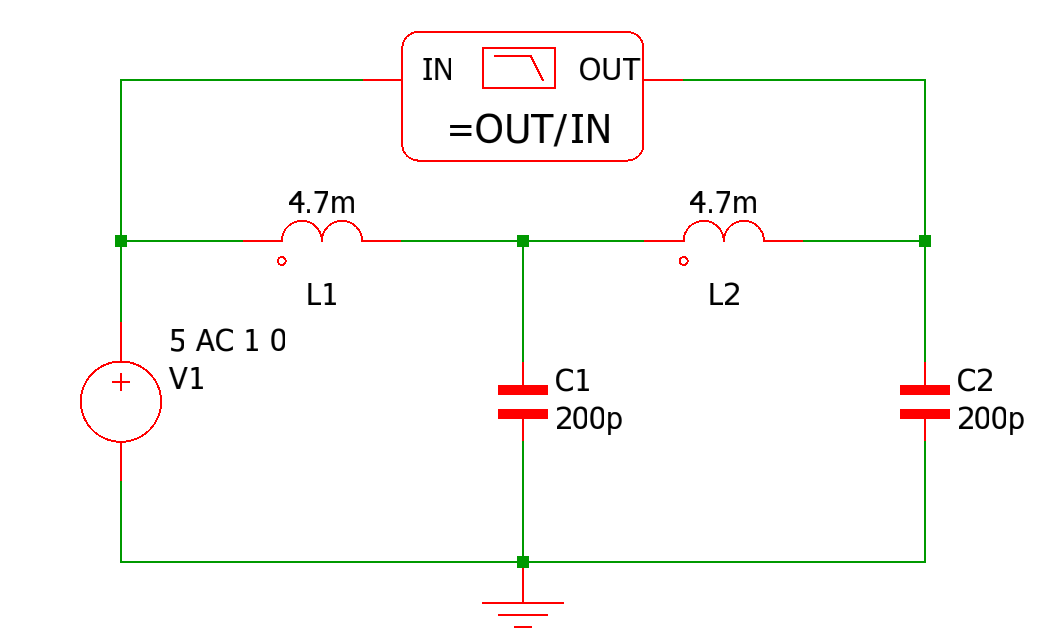
\includegraphics[width=\textwidth]{pictures/schemaideale_vero.png}
	\label{fig:largenenough}
	\caption{\label{lul} \small LCLC simulato}
\end{figure}

Si nota nei grafici nella pagina succesiva come il circuito si comporti come aspettato, con due poli nelle seguenti frequenze
\begin{align}
&\omega_1 = 101.859 \; [kHz]\\
&\omega_2 = 265.461 \; [kHz]
\end{align}

Valori decisamente compatibili con quelli calcolati dalla teoria.

Notiamo inoltre come, per tali valori di $L$ e $C$ dati, si abbia un filtro \textbf{Passa-Basso} a banda passante estremamente larga, fino oltre i $400 \; [kHz]$

\begin{figure}[!htb]
	\centering
	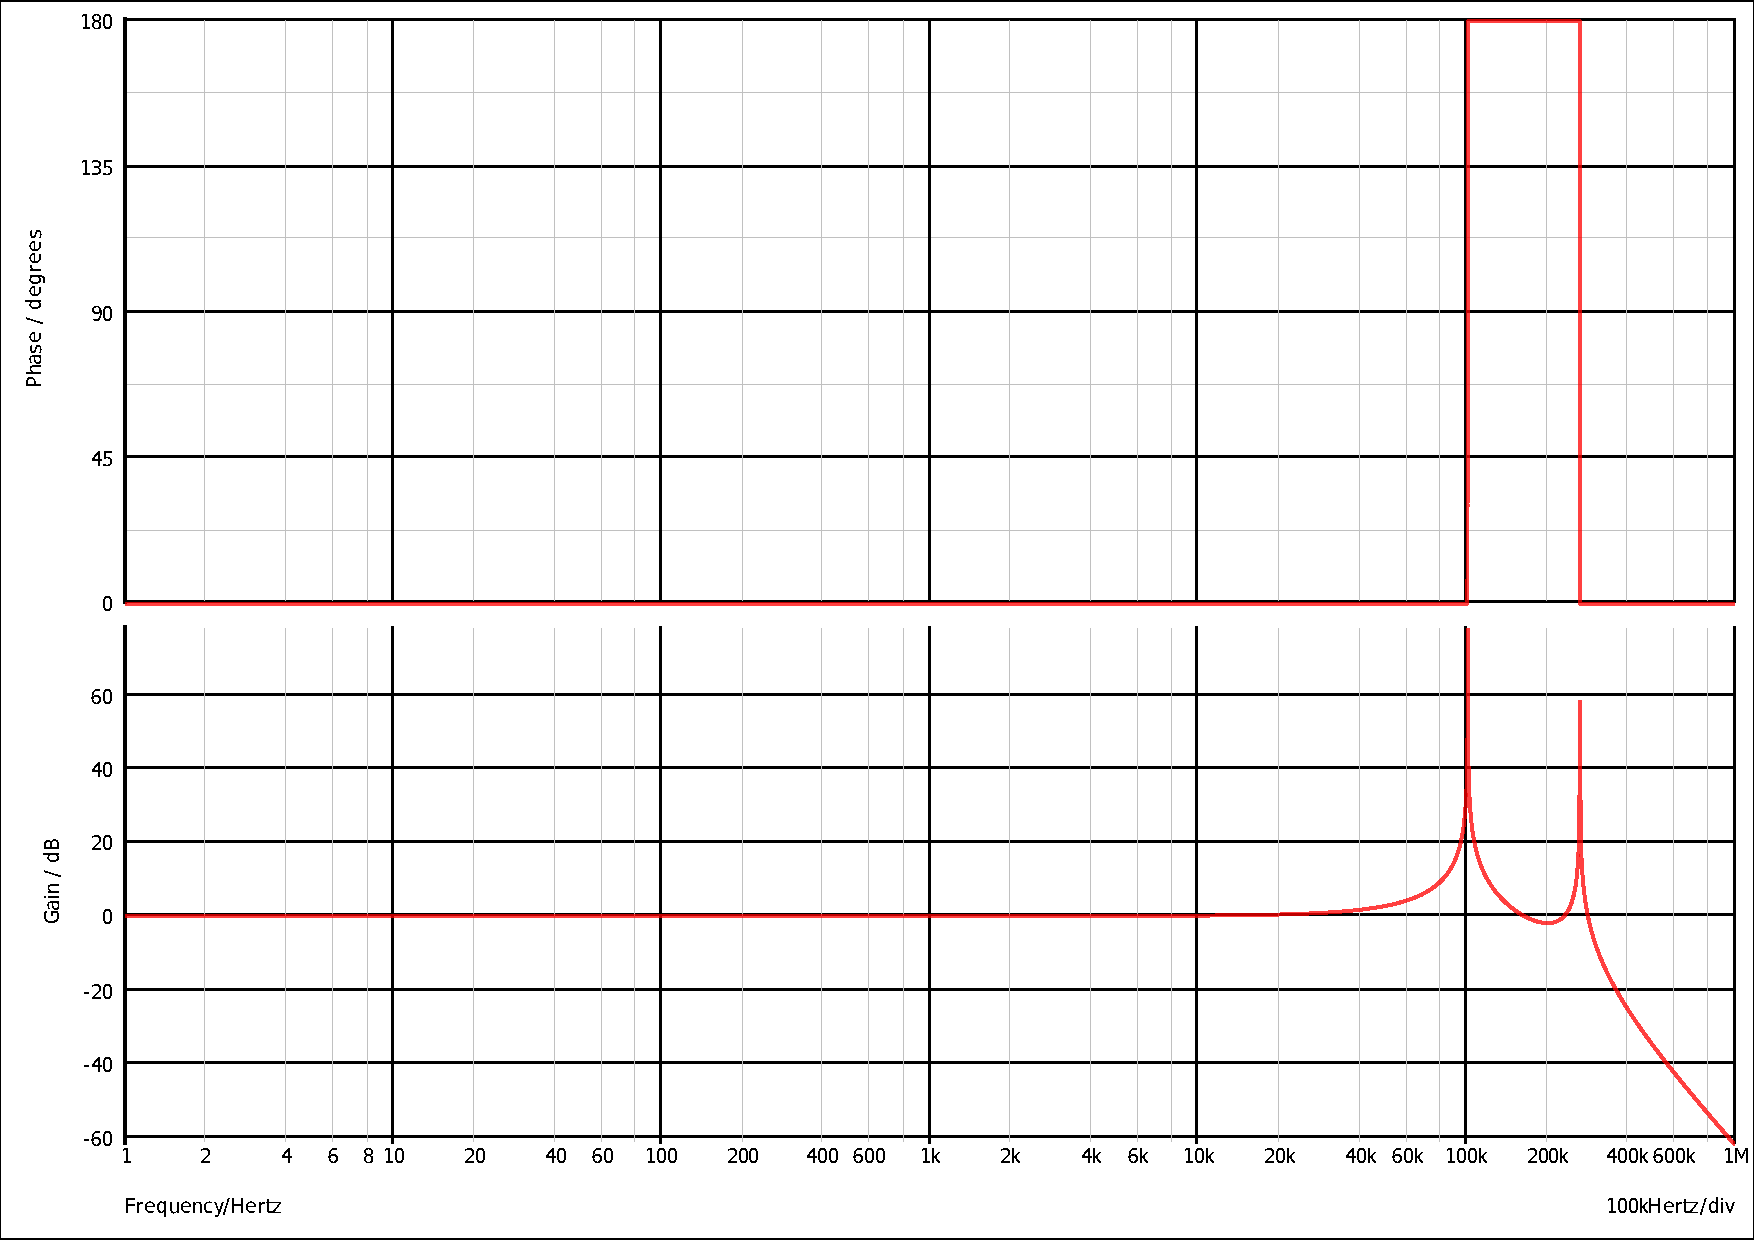
\includegraphics[width=.8\textwidth]{pictures/LCLC_non_adattato.pdf}
	\label{fig:largenenough}
	\caption{\label{lul} \small Diagrammi di Bode per circuito non adattato}
\end{figure}

\begin{figure}[!htb]
	\centering
	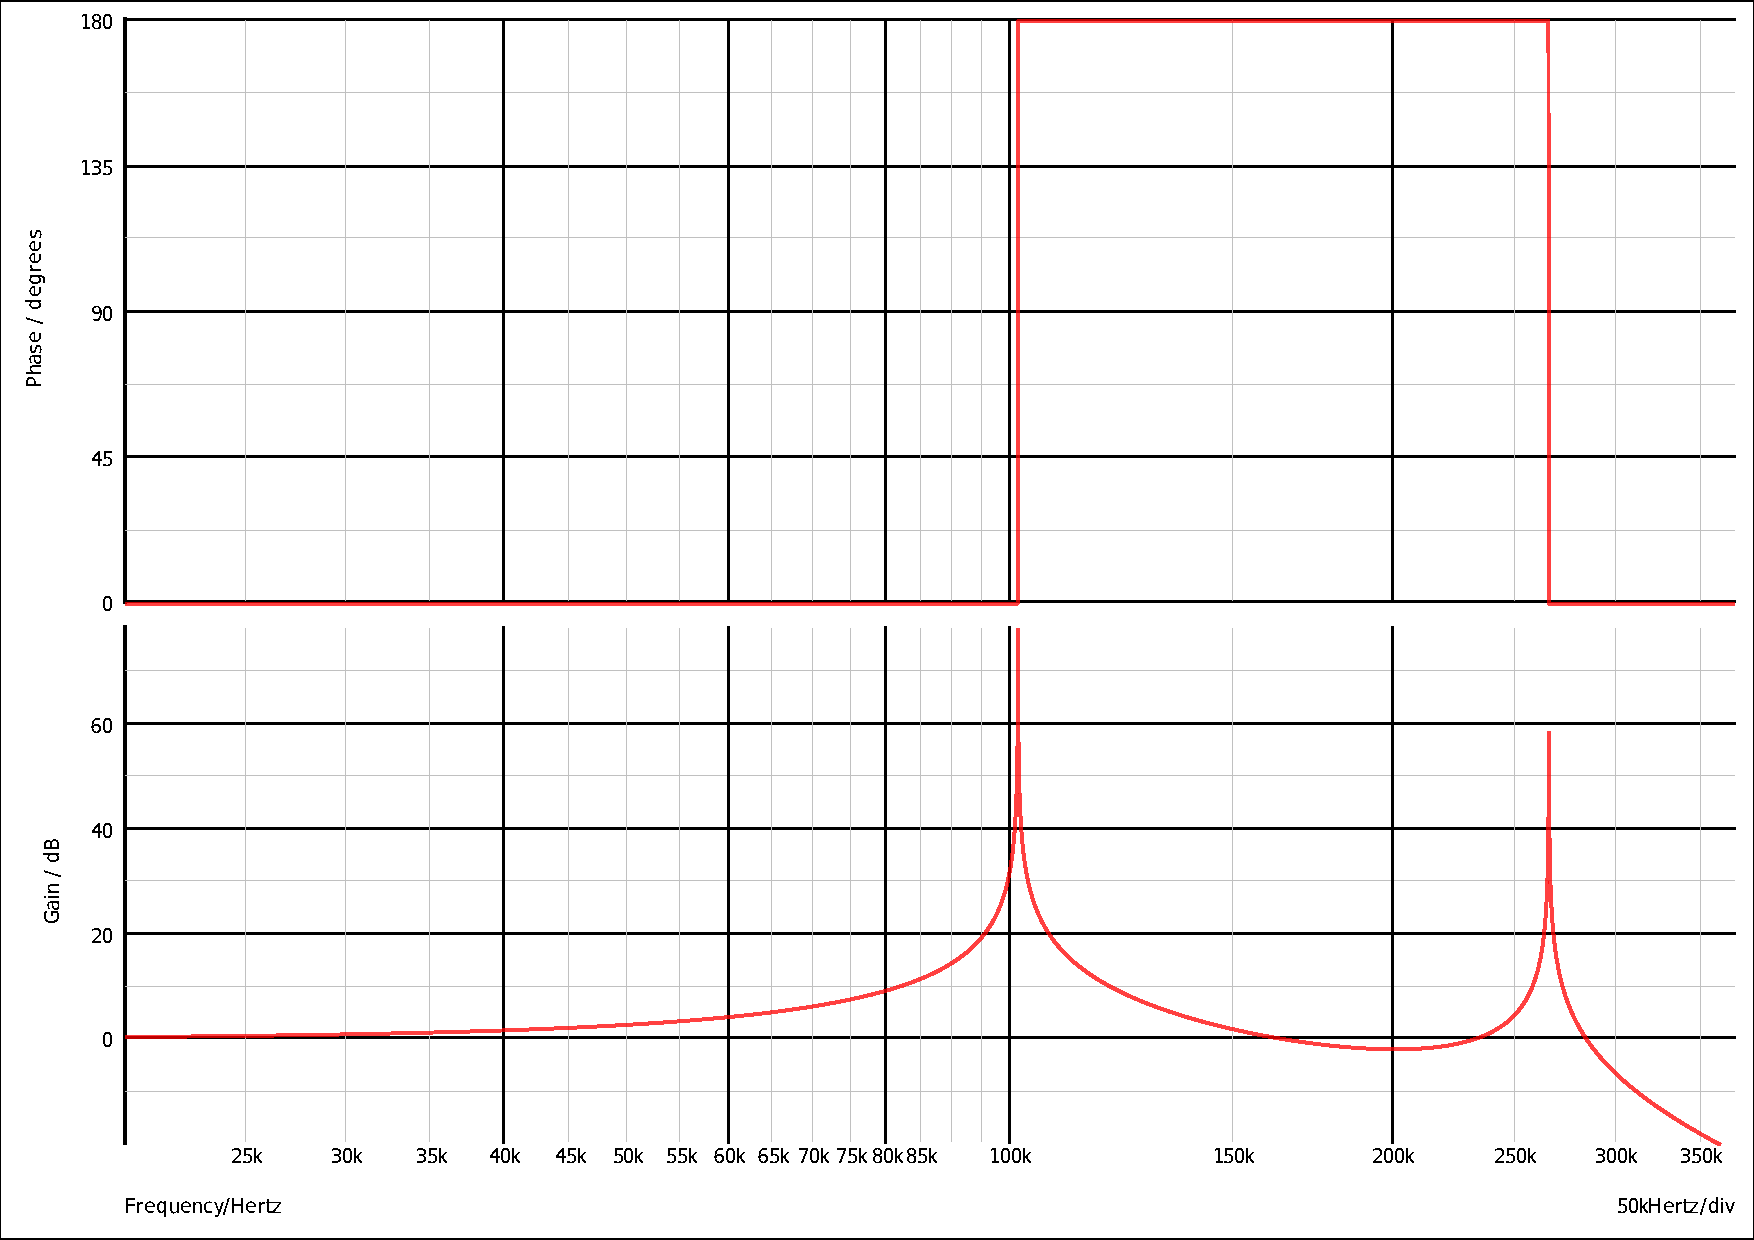
\includegraphics[width=.8\textwidth]{pictures/LCLC_non_adattato_zoom_osc.pdf}
	\label{fig:largenenough}
	\caption{\label{lul} \small Zoom in vicinanza dei poli}
\end{figure}

\clearpage


\subsection{Simulazione del circuito ideale adattato in potenza}

Dati i valori di $L$ e $C$, per avere adattamento in potenza avremo bisogno di una resistenza di valore
\begin{align}
R_L = \sqrt{\frac{4.7 \cdot 10^{-3}}{2 \cdot 10^{-10}}} \simeq 4.8 \; [k\Omega]
\end{align}

Il nostro circuito diventerà quindi
\begin{figure}[!htb]
	\centering
	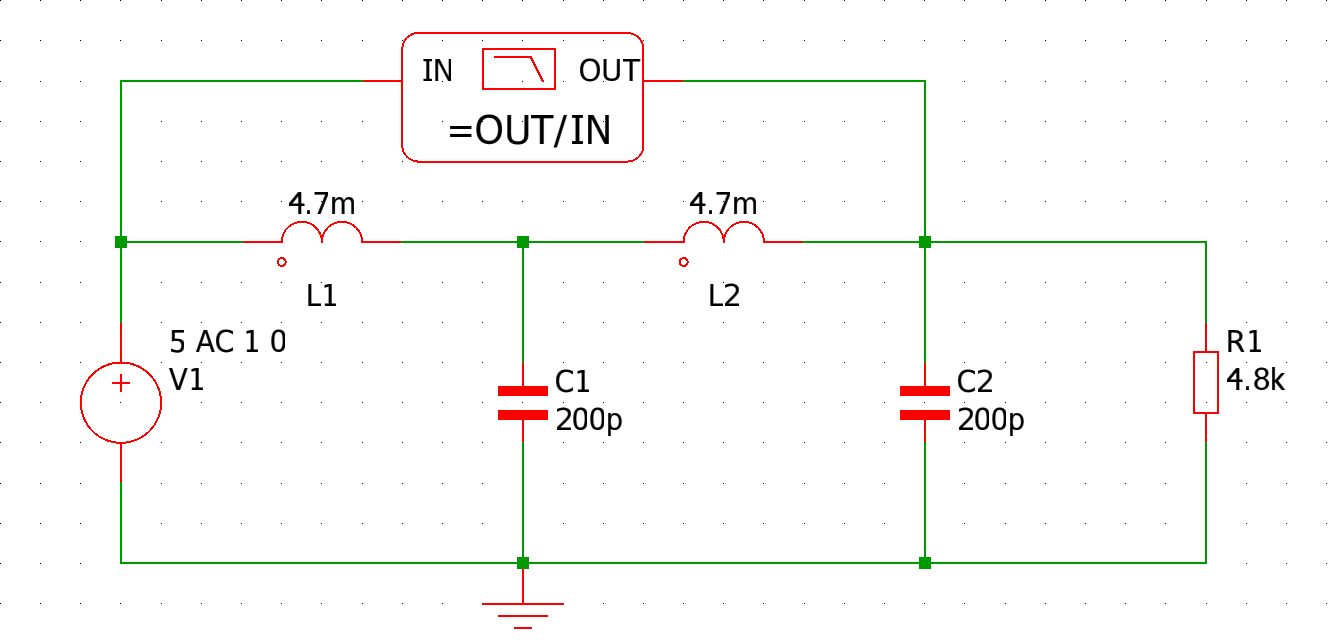
\includegraphics[width=\textwidth]{pictures/schemaideale_vero_adattato.png}
	\label{fig:largenenough}
	\caption{\label{lul} \small LCLC adattato}
\end{figure}

Notiamo nei seguenti diagrammi di Bode come il circuito si comporti in modo alaogo al caso non adattato con eccezione delle esplosioni in prossimità dei poli, ora notevolmente ammortizzate dal carico.

\begin{figure}[!htb]
	\centering
	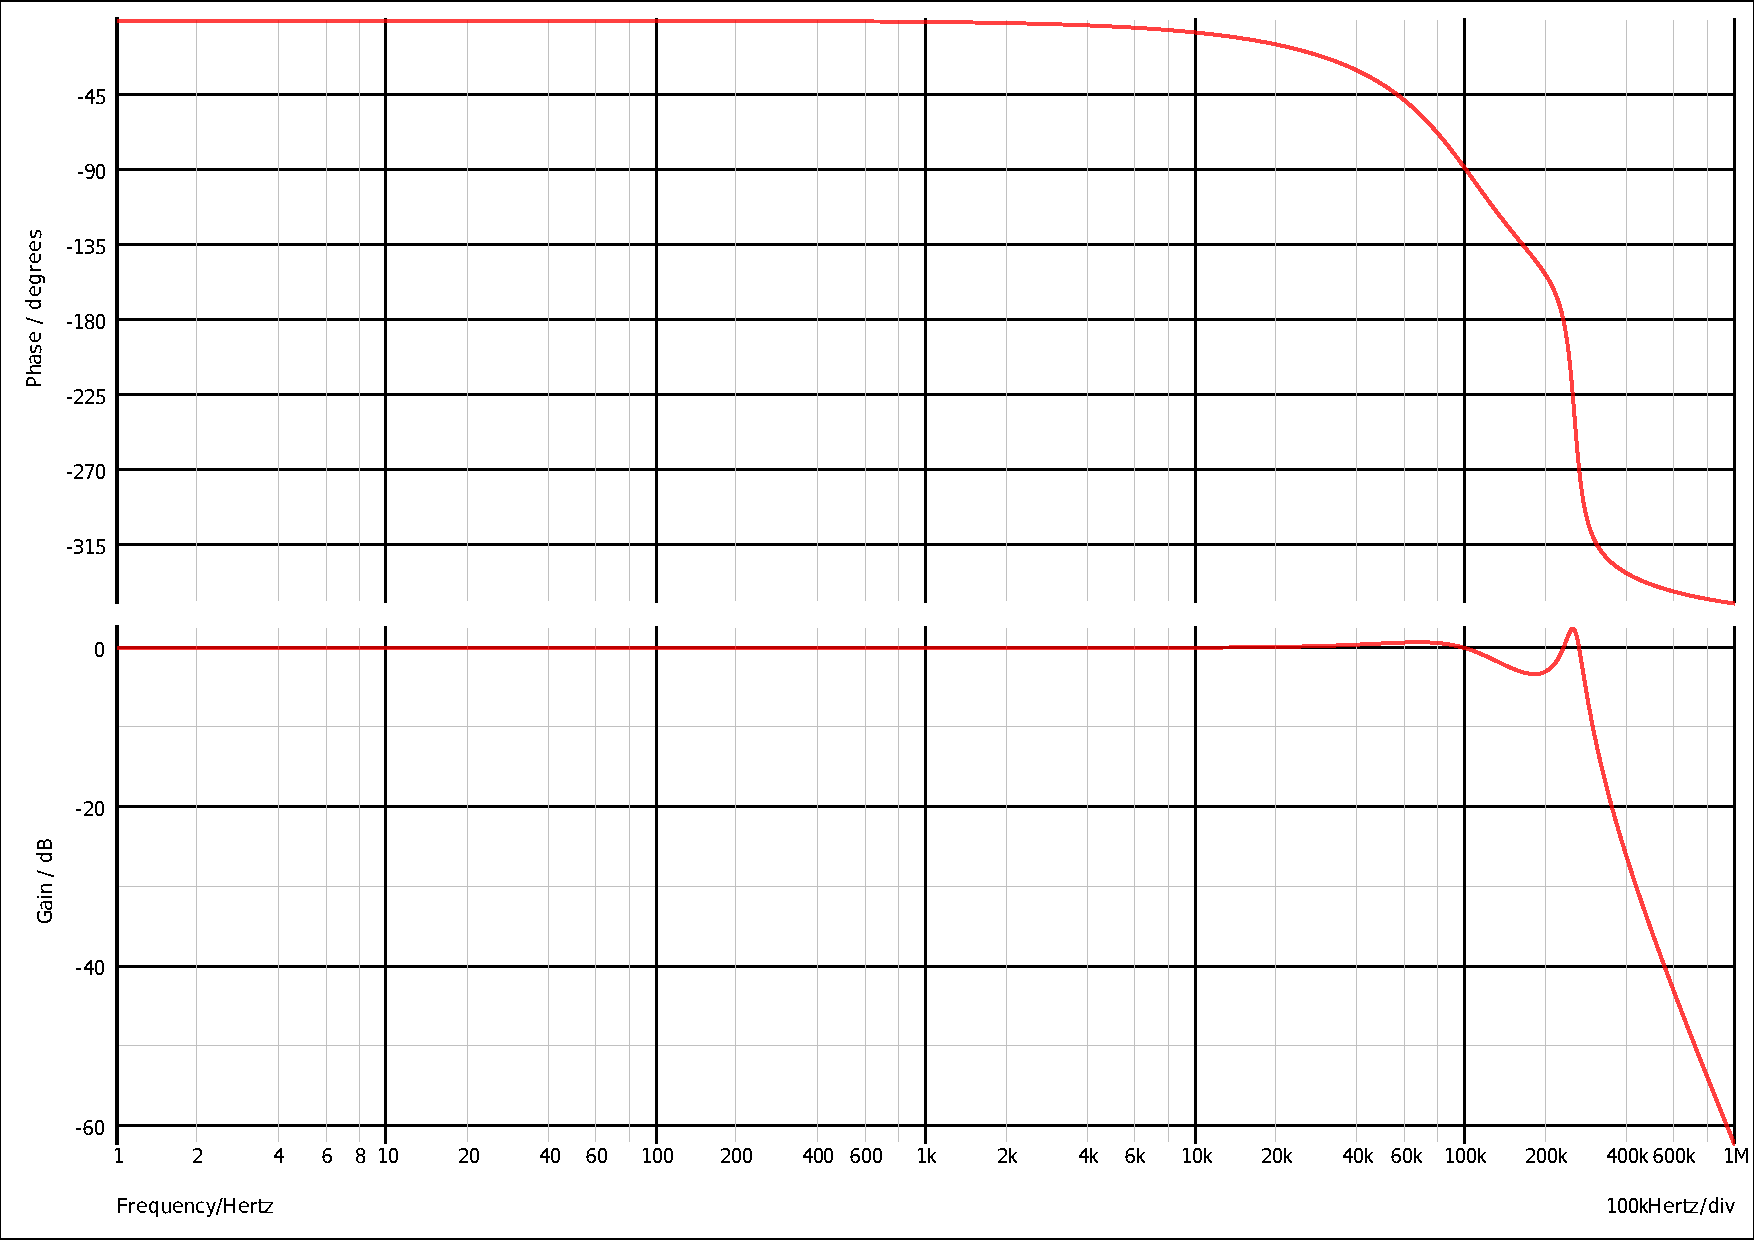
\includegraphics[width=.8\textwidth]{pictures/LCLC_adattato.pdf}
	\label{fig:largenenough}
	\caption{\label{lul} \small Diagrammi di Bode per circuito non adattato}
\end{figure}

\begin{figure}[!htb]
	\centering
	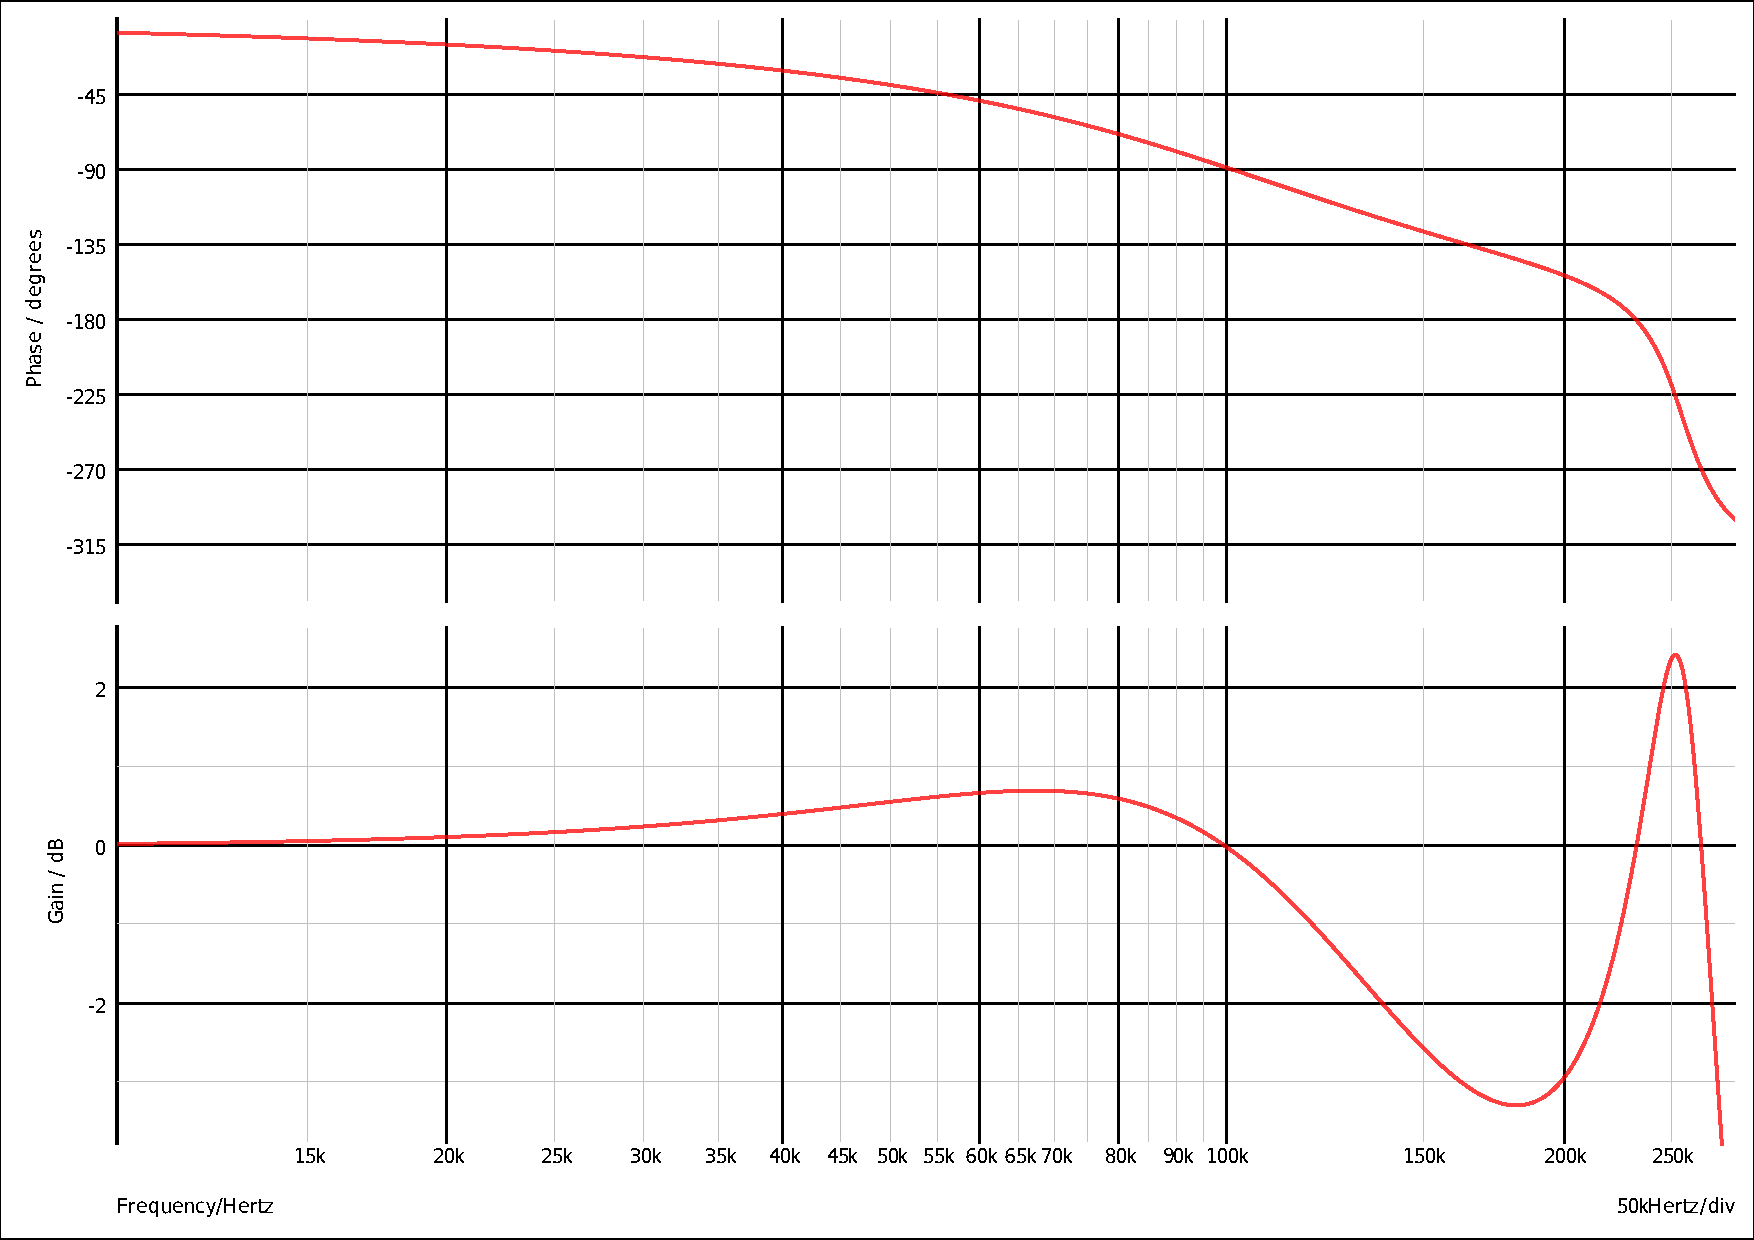
\includegraphics[width=.8\textwidth]{pictures/LCLC_adattato_zoom_osc.pdf}
	\label{fig:largenenough}
	\caption{\label{lul} \small Zoom in vicinanza dei poli}
\end{figure}

\end{document}          
